\chapter{\IfLanguageName{dutch}{Proof of Concept}{Proof of Concept}}%
\label{ch:proof-of-concept}
\subsection{Benodigdheden}%
\label{subsec:benodigdheden}
Omdat alle platformen cloud-based zijn, is er een laptop en een internetverbinding nodig om de Proof of Concept uit te voeren. Vervolgens heb je ook 
een account nodig op de drie platformen; Softr, Stacker en Bubble. Deze drie platformen bieden dan ook een gratis versie aan waardoor er geen kosten aan verbonden zijn. Vervolgens zal je ook 
nog een account nodig hebben op AirTable en MAKE.com die ook een gratis versie aanbieden.

\subsection{Uitvoer van de Proof of Concept}%
\label{subsec:uitvoer-proof-of-concept}

\subsubsection{Programmeur}%
\label{subsubsec:programmeur}
Voor de drie platformen te laten testen door een programmeur zal natuurlijk niet alle 3 de platformen tegelijkertijd 
kunnen getest worden, daarom zal de programmeur eerst beginnen met Softr. 
Zoals eerder vermeld zal de programmeur een feedback app moeten maken.
\\
\\
\textbf{1. Softr}
\\
Hiervoor moet hij eerst een account maken op Softr en op AirTable om de app te kunnen maken. 
Daarna kom je terecht op een overzichtelijke dashboard waar je de keuze hebt om templates te kiezen maar 
ook je eigen app te maken van nul of met AI. Bij het ontwikkelen van de app ervaarden de programmeur één probleem. 
Dit probleem was een error dat hij kreeg bij het snel verwijderen van componenten waardoor de pagina zich herstartte. 
Vervolgens merkte hij op dat de app kan hersteld worden aan de hand van de App History waarbij je terug kunt gaan 
naar een bepaalde snapshot. De programmeur heeft dan uiteindelijk de feedback app 
kunnen maken in exact 41 minuten en 54 seconden, de besteden tijd in AirTable is niet inbegrepen. 
Dit was zonder het gebruik van de AI, die Softr aanbiedt om je pagina’s voor u te maken. Vervolgens vond 
de programmeur de aantal integraties dat hij zag redelijk gelimiteerd maar de integratie met Airtable was 
zeer goed en simpel. Je kon wel helaas geen twee tabellen van de database connecteren op 1 formulier. 
Ook zag het er zeer eenvoudig uit om MAKE.com te gebruiken, maar doordat je in Softr geen 2 verschillende connecties 
kan leggen op één knop heeft de programmeur enkel AirTable gebruikt.
\\
\\
Hieronder zie je de AirTable database dat de programmeur heeft gemaakt en hoe het gebruikmaken van AirTable in Softr plaatsnam.
\\
\\
\begin{figure}[H]
    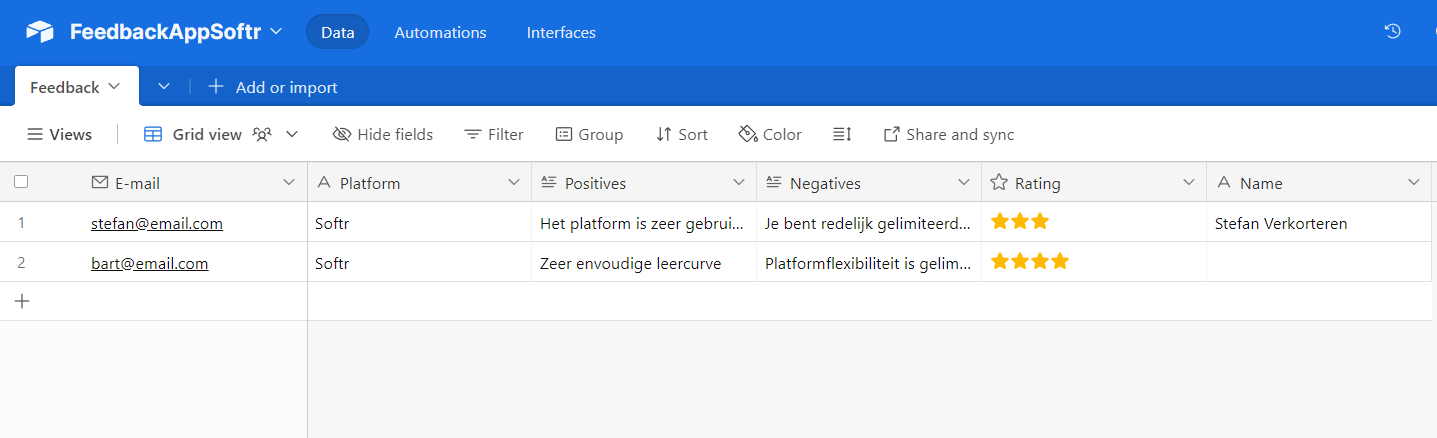
\includegraphics[scale=0.5]{softr/database-airtable-softr.png}
    \caption[Airtable database voor Softr]{Airtable database voor Softr\\\textcopyright\ Joeri Verhelst}
    \label{fig:database-airtable-softr}
\end{figure}
\begin{figure}[H]
    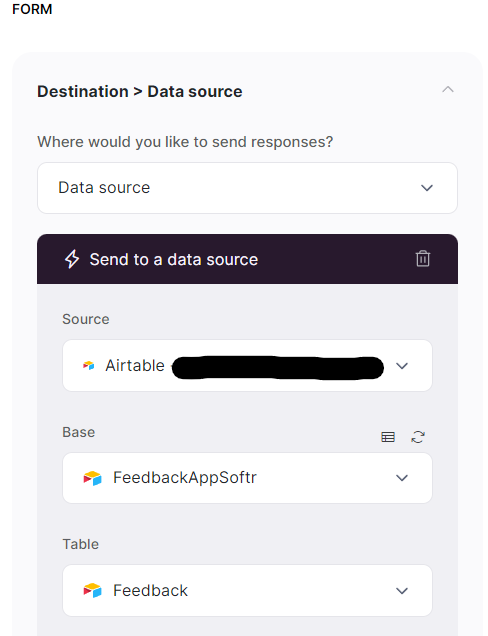
\includegraphics[scale=0.5]{softr/airtable-connectie.png}
    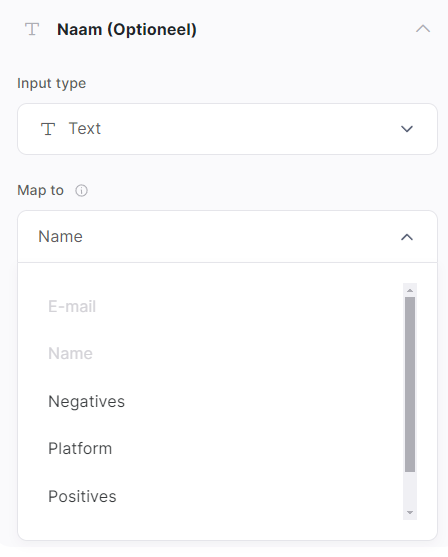
\includegraphics[scale=0.5]{softr/connectie-leggen-aan-airtable-velden.png}
    \caption[Airtable connectie met Softr]{Airtable connectie met Softr\\\textcopyright\ Joeri Verhelst}
    \label{fig:database-airtable-softr-connectie}
\end{figure}

Op vlak van platformflexibiliteit vond de programmeur het zeer matig. 
Want je kan namelijk geen meerdere acties plaatsen op een knop. 
Daarbij is het layout aanpassen van een componenten ook zeer beperkt zoals een component een border radius of shaduw geven is niet mogelijk. 
Wat de programmeur wel zeer tof vond is dat je de optie hebt om eigen custom componenten te maken via high-code en ook templates kon gebruiken.
\\
\\
Softr scoorde wel heel goed op gebruiksvriendelijkheid volgens de programmeur. 
Hij vond het zeer overzichtelijk en kon er snel mee omgaan. 
Juist was het niet mogelijk om individuele delen van een component aan te duiden om snel aan te passen. 
Alle wijzingen moeten namelijk gebeuren in het rechterpaneel waardoor je telkens moest zoeken naar het deel dat je wou aanpassen. 
Ook was je verplicht om een één template aan te duiden als startpagina bij het kiezen om een app te maken van nul, wat zeer apart was. 
\\
\\
\begin{figure}[H]
    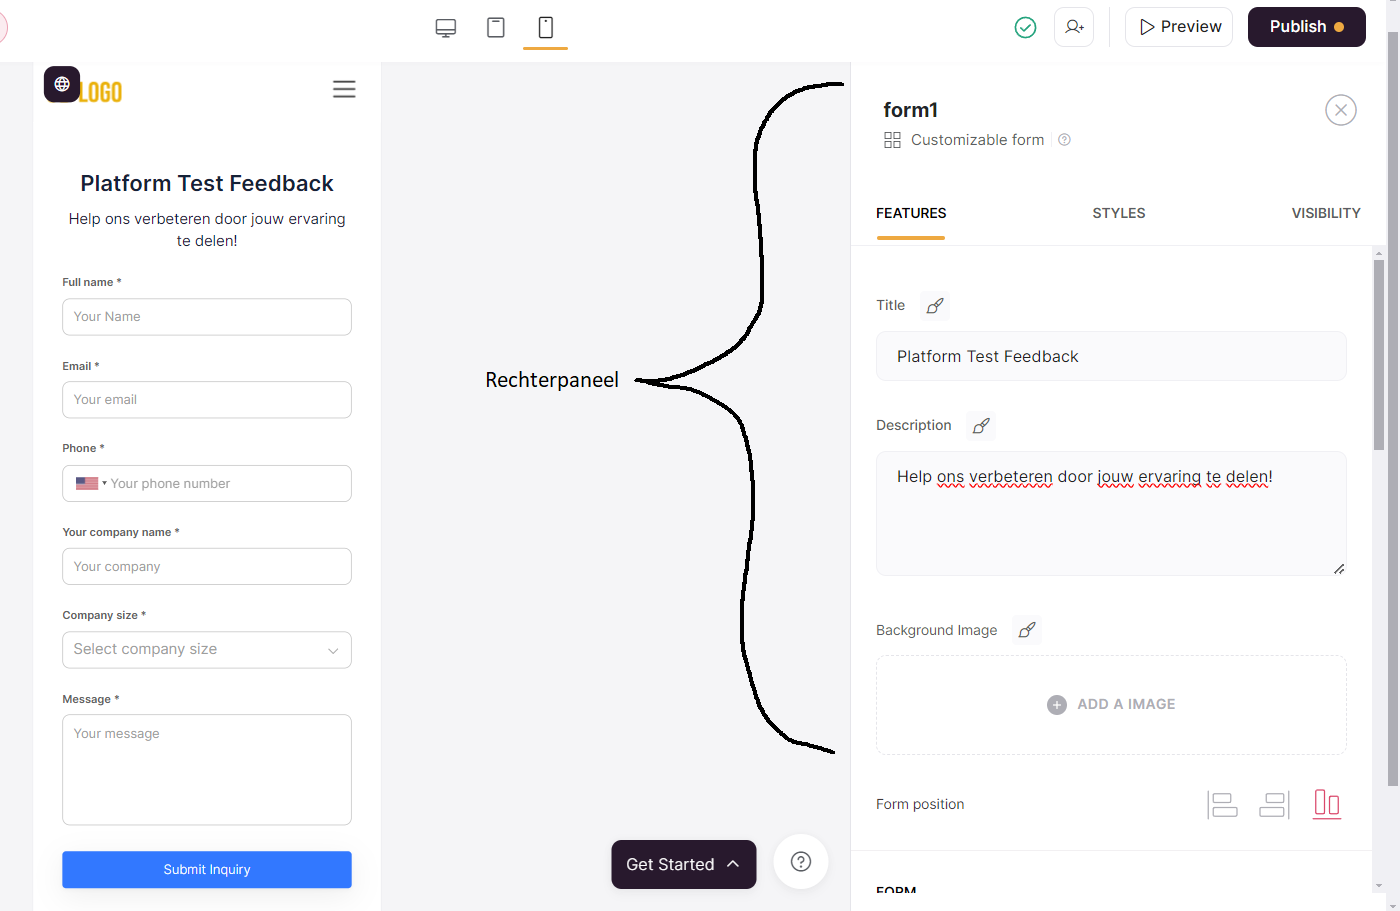
\includegraphics[scale=0.5]{softr/rechter-paneel.png}
    \caption[Het rechterpaneel van Softr]{Het rechterpaneel van Softr\\\textcopyright\ Joeri Verhelst}
    \label{fig:softr-rechterpaneel}
\end{figure}
\paragraph*{Eindresultaat}
Hieronder kunt u het eindresultaat zien van de feedback app dat gemaakt is in Softr. Door de beperkte platformflexibiliteit kon men namelijk het voorbeeld niet volledig namaken. 
Vervolgens is er ook gebruik gemaakt van een eigen component voor de titel en ondertitel. Dit component werd geschreven in HTML5 met Bootstrap.
\\
\\

\begin{figure}[H]
    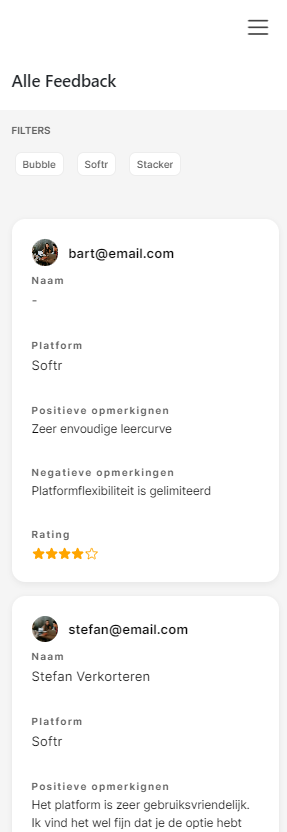
\includegraphics[scale=0.75]{softr/feedbacklijst-softr.png}
    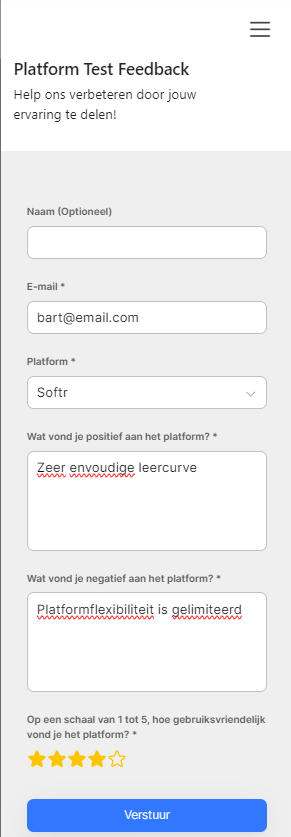
\includegraphics[scale=0.75]{softr/formulier-gemaakt-softr.png}
    \caption[Feedback app gemaakt in Softr]{Feedback app gemaakt in Softr\\\textcopyright\ Joeri Verhelst}
    \label{fig:softr-feedback-app}
\end{figure}

\paragraph*{Beoordeling}
De programmeur geeft deze app een score van 4 op 5 doordat je kon opmerken dat het platform wel redelijk gelimiteerd is, maar wel de mogelijkheid had om eigen componenten te maken. 
Hierdoor kon de programmeur achterhalen dat het maken complexe apps een echte uitdaging zou zijn met Softr, 
door de beperkte platformflexibiliteit.
\\
\\
\textbf{2. Bubble}
\\
Bij Bubble was het maken en starten van een app gelijkaardig aan Softr. Het platform op zich was snel en vlot om mee te werken. Maar bij het testen van een actie op een knop
kon het proces soms eventjes duren vooraleer de actie werd uitgevoerd. Vervolgens was het wel mogelijk bij bubble om op een knop meerdere acties te plaatsen waardoor men ook 
bij dit platform een mail versturen naar de gebruiker die feedback heeft gegeven. Hieronder kunt u dan ook de scenario vinden dat gemaakt is in MAKE.com.
\\
\begin{figure}[H]
    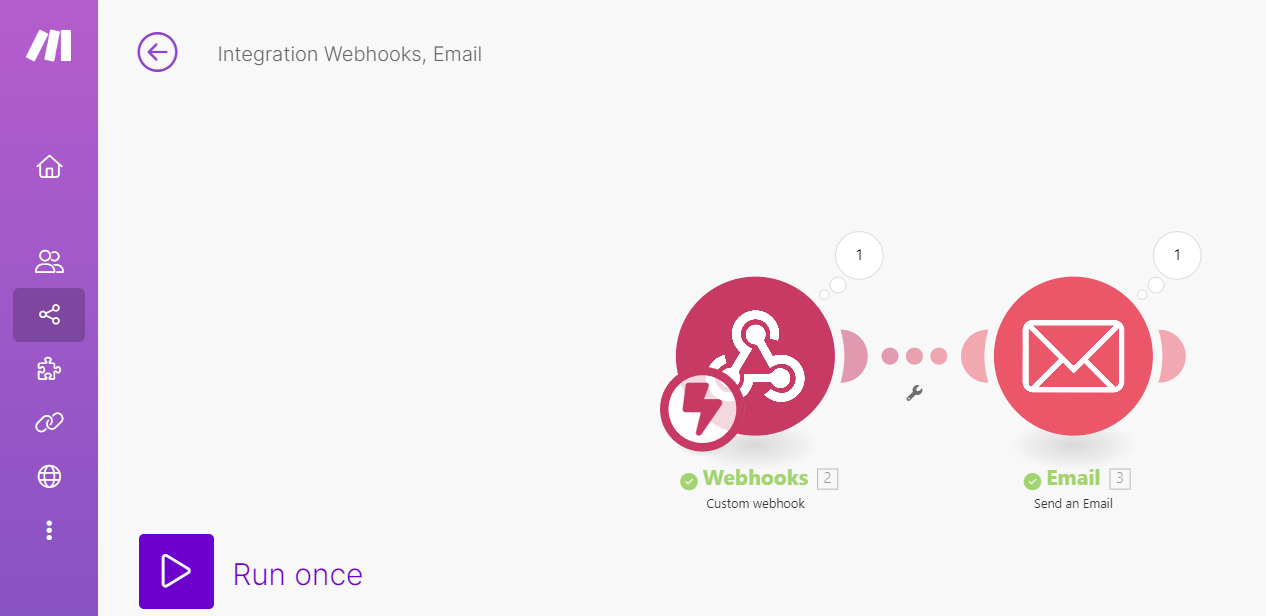
\includegraphics[scale=0.5]{bubble/make-scenario.png}
    \caption[MAKE.com scenario voor het versturen van e-mail]{MAKE.com scenario voor het versturen van e-mail\\\textcopyright\ Joeri Verhelst}
    \label{fig:make-scenario-bubble}
\end{figure}
Het integreren met Airtable en MAKE.com was in het begin zeer verwarrend voor de programmeur. Het duurde toch wel eventjes vooraleer hij doorhad hoe hij de connectie moest leggen.
Na het zoeken naar de documentatie was het duidelijk dat je een personal acces token moet maken op Airtable om dit dan te gebruiken in Bubble. De tijd dat de programmeur nodig had 
om te integreren was 36 minuten en 3 seconden. Hieronder vind u dan ook de AirTable database dat de programmeur heeft gemaakt en de integratie met Bubble.
\\
\\


\begin{figure}[H]
    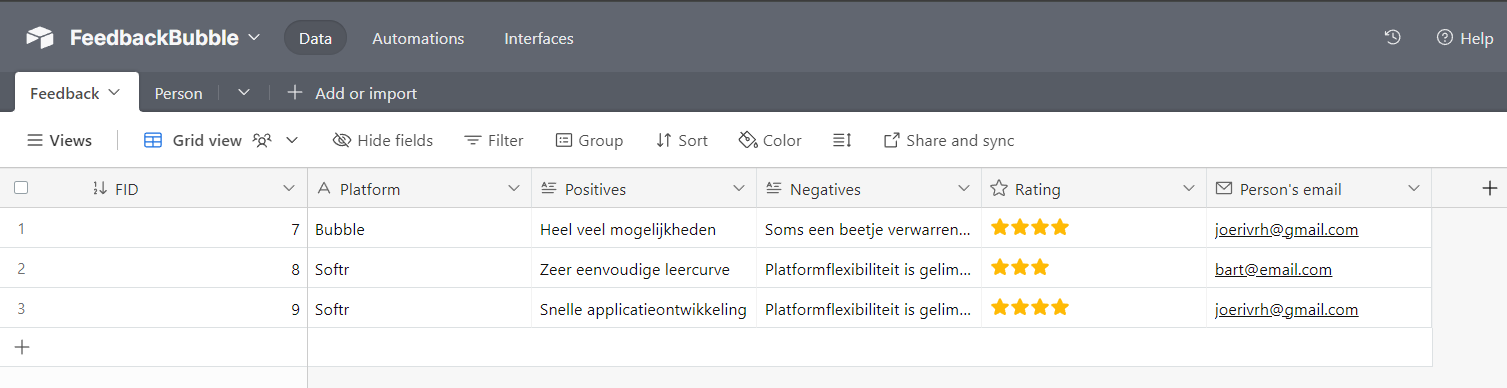
\includegraphics[scale=0.5]{bubble/AirTable-Bubble.png}
    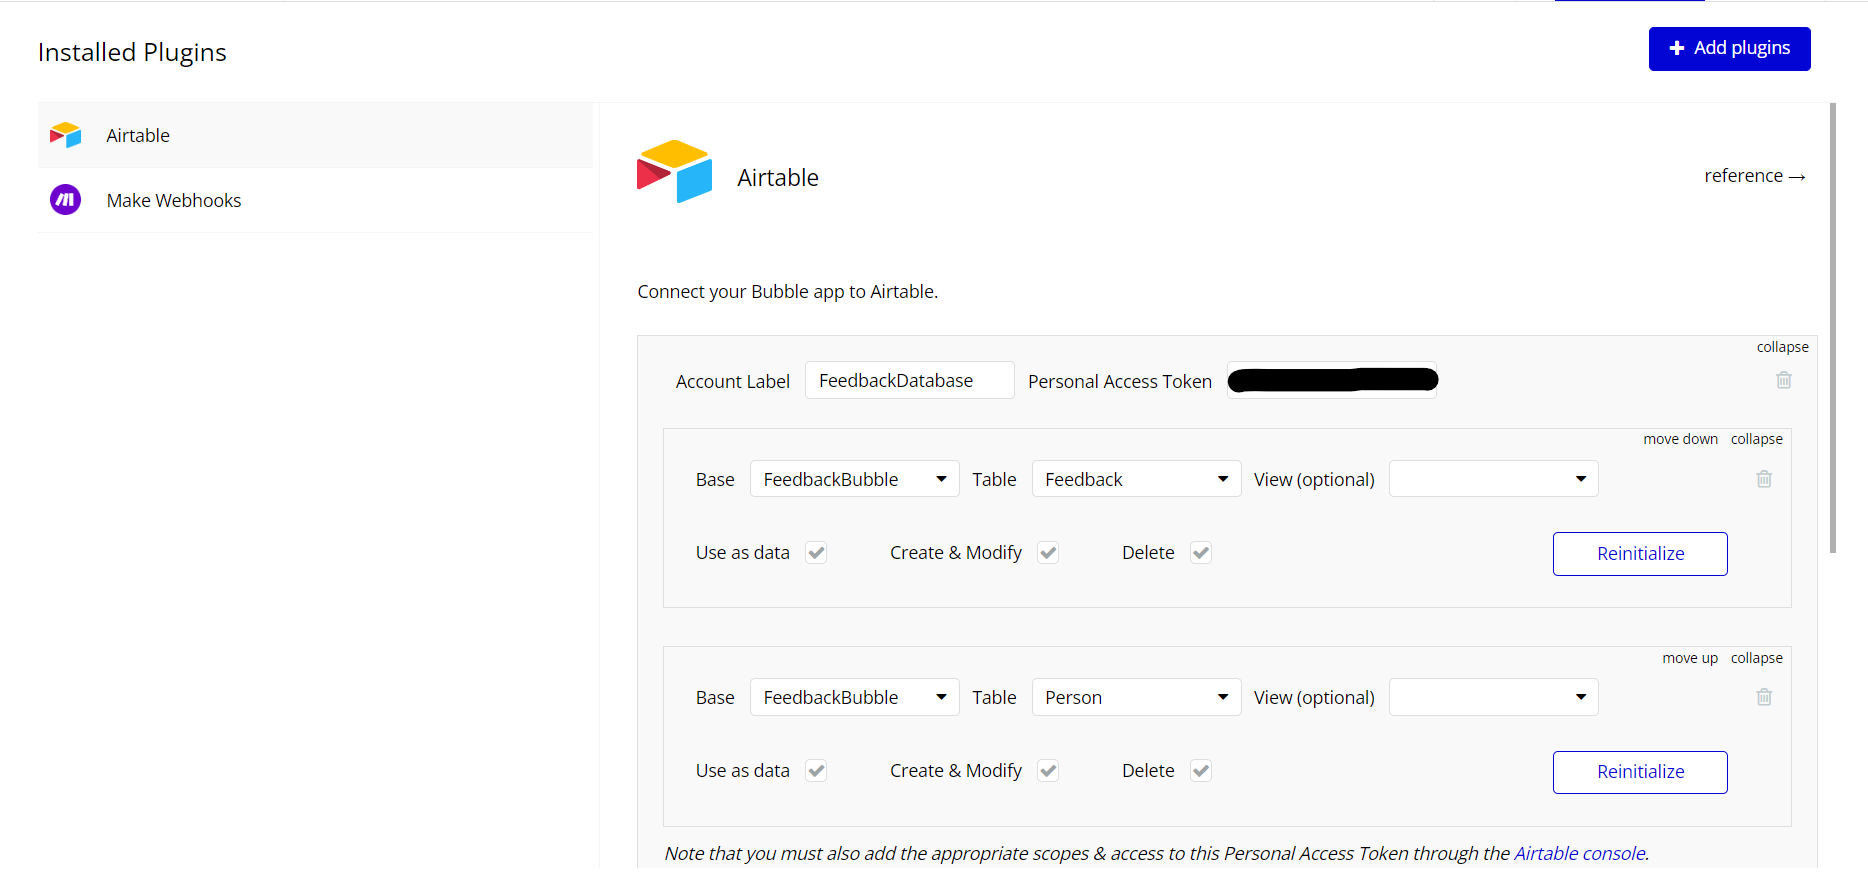
\includegraphics[scale=0.4]{bubble/integratie-airtable.png}
    \caption[Integratie en Airtable database voor Bubble]{Integratie en Airtable database voor Bubble\\\textcopyright\ Joeri Verhelst}
    \label{fig:airtable-bubble}
\end{figure}
Op vlak van platformflexibiliteit was Bubble zeer goed. Je kon namelijk alles aanpassen van een component zoals de border radius, schaduw, kleur, enzovoort. 
De programmeur vond het ook duidelijk dat je met dit platform complexe apps zou kunnen maken. Daarnaast was het eerst zoeken naar hoe je acties moest plaatsen op een knop.
Je moet namelijk naar een aparte sectie gaan die alle bedrijfslogica bevat. Dit was eerst wat verwarrend voor de programmeur. De flow's of meer specifiek de acties dat je bijvoorbeeld kan doen op een 
knop was zeer flexibel, want dit zorgde ervoor dat je op een knop zowel een actie kan doen met Airtable als met MAKE.com.
\\

\begin{figure}[H]
    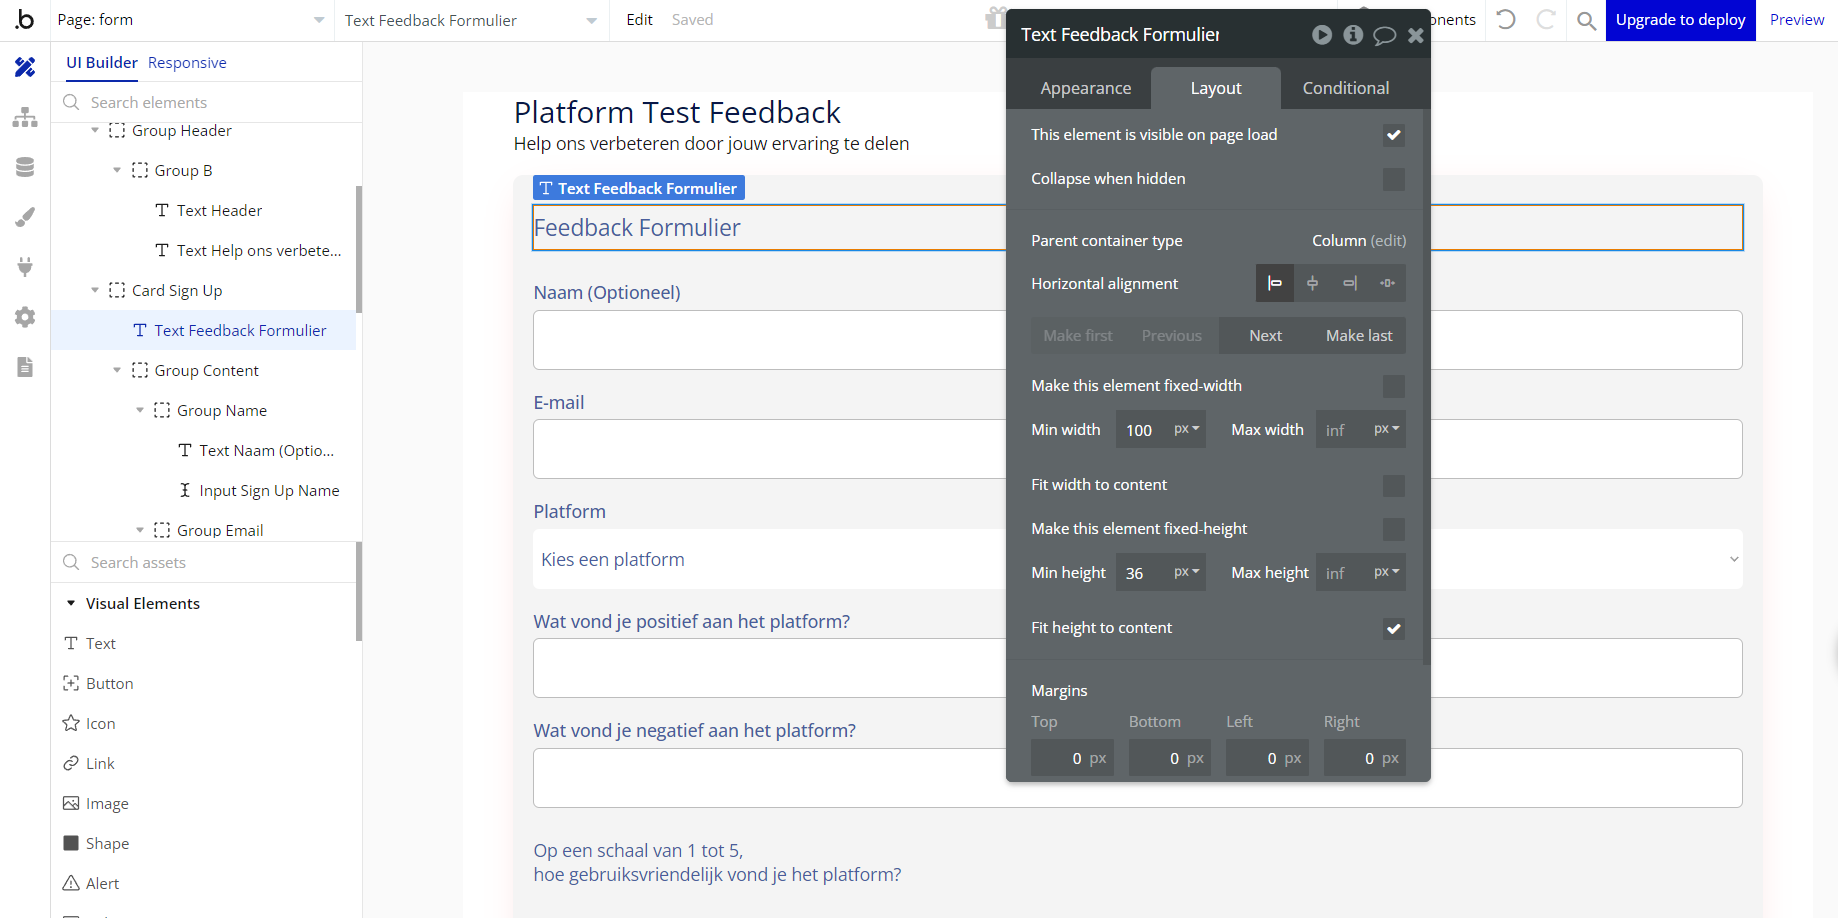
\includegraphics[scale=0.4]{bubble/element-details.png}
    \caption[Details van een element in Bubble]{Details van een element in Bubble\\\textcopyright\ Joeri Verhelst}
    \label{fig:element-bubble}
\end{figure}
De gebruiksvriendelijkheid van de app is goed. Je komt namelijk terecht
op een scherm waarbij je kan kiezen om een app te ontwikkelen via AI of zelf van nul te beginnen. 
Vervolgens heb je de optie om direct plugins te intalleren zoals MAKE.com en Airtable. Daarna moet je de kleuren kiezen van de app.
Bij het klikken op een component krijg je direct de opties te zien die je kan aanpassen, wat zeer handig is want dit geldt voor ook delen in het component. Helaas 
kan je de live data wel niet zien in de editor maar wel bij het previewen van de app.
\\
\\
\paragraph*{Eindresultaat}
De programmeur heeft de app kunnen maken in 1 uur en 52 minutren. De oorzaak hiervan was omdat het vaak wel zoeken was hoe iets in elkaar zat, dit gelde ook bij het integreren van plugins.
Het maken van de feedbacklijst duurde het langste, namelijk 45 minuten en 18 seconden doordat het niet duidelijk was hoe je de data van Airtable moest tonen in een lijst.
Uiteindelijk is de app dat gemaakt is in Bubble zeer gelijkaardig aan het voorbeeld, door de vrijheid die Bubble beschikt. Hieronder vind u dan ook het eindresultaat van de feedback app.
\\
\begin{figure}[H]
    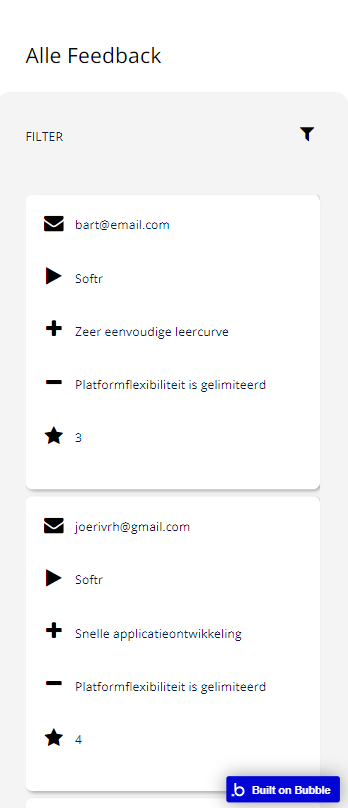
\includegraphics[scale=0.5]{bubble/feedback-lijst-bubble.png}
    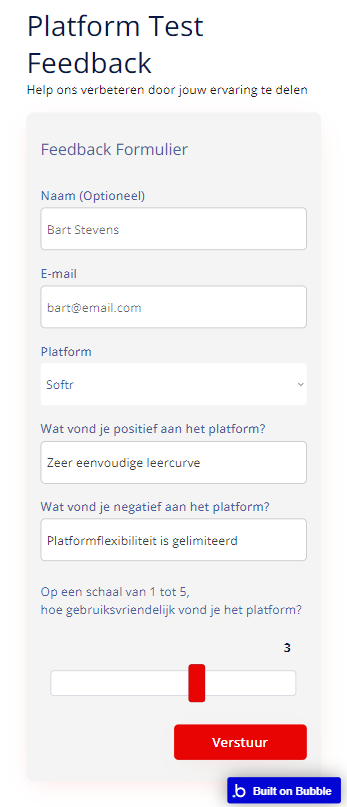
\includegraphics[scale=0.5]{bubble/formulier-resultaat-bubble.png}
    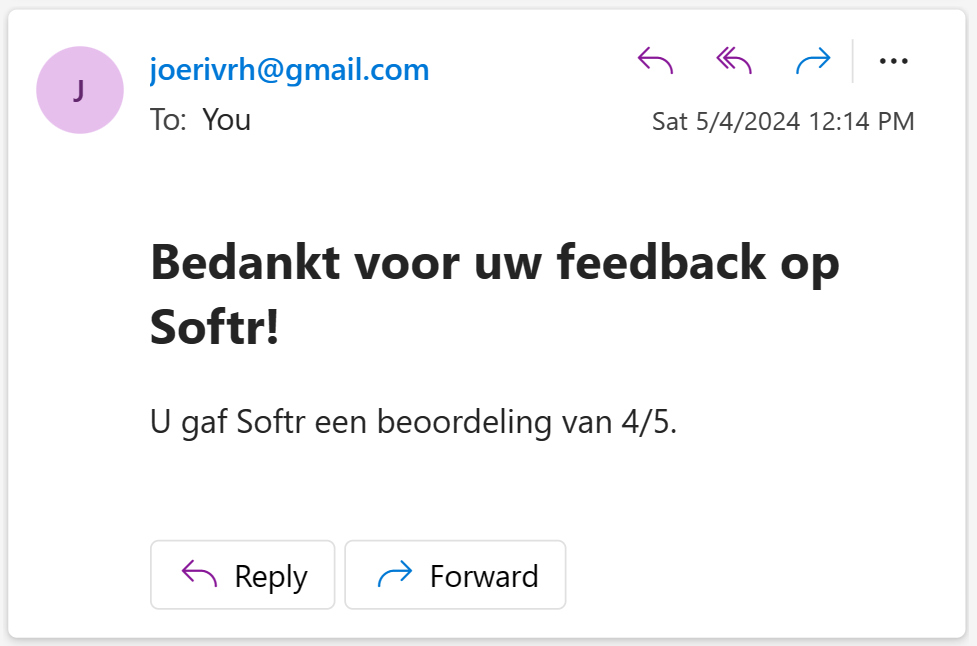
\includegraphics[scale=0.5]{bubble/ontvangen-email-bij-formulier-bubble.png}
    \caption[Feedback app gemaakt in Bubble]{Feedback app gemaakt in Bubble\\\textcopyright\ Joeri Verhelst}
    \label{fig:feedback-app-bubble}
\end{figure}

\paragraph*{Beoordeling}
De beoordeling dat deze app heeft gekregen is 4.5 op 5. Dit komt omdat het platform zeer flexibel is. 
De beoordeling was net geen 5 op 5 omdat het soms wel zoeken was hoe je iets moest doen.
\\
\\
\textbf{3. Stacker}
\\
Bij Stacker was het proces voor het maken van een app zeer strikt en kon je niet veel aanpassen. Je moest namelijk eerst een account maken met een bedrijfsaccount.
Daarna werd er direct gevraagd om een databron te connecteren met Stacker. Hiervoor nam de programmeur AirTable waarbij het connecteren zeer snel en vlot verliep, door de duidelijke documentatie.
Helaas merkte de programmeur op, bij het ontwikkelen van de feedback app, dat het niet mogelijk was om MAKE.com te integreren met Stacker.
\\
\\
Hieronder zie je de AirTable database dat de programmeur heeft gemaakt.
\\
\\
\begin{figure}[H]
    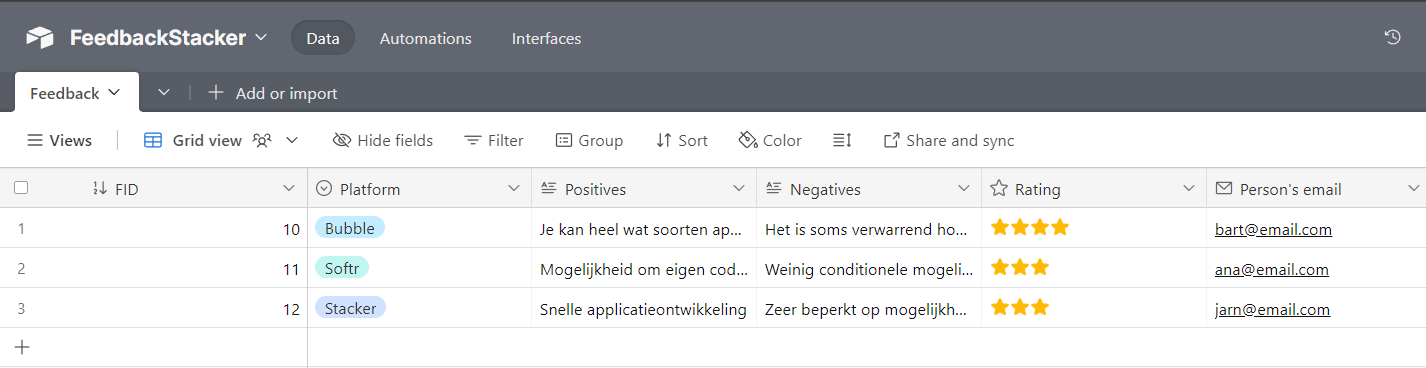
\includegraphics[scale=0.5]{stacker/airtable_stacker.png}
    \caption[Airtable database voor Stacker]{Airtable database voor Stacker\\\textcopyright\ Joeri Verhelst}
    \label{fig:airtable-stacker}
\end{figure}
Op vlak van platformflexibiliteit had je heel weinig vrijheid om je app aan te passen. Je kon namelijk niet de kleur kiezen van componenten want de kleuren worden gekozen
op basis van je bedrijfskleur. Daarnaast heb je ook weinig keuze in componenten. De programmeur vond dat dit platform meer bedoelt is voor het maken van CRM's en portals in plaats van 
mobiele of complexe apps.
\\
\\

\begin{figure}[H]
    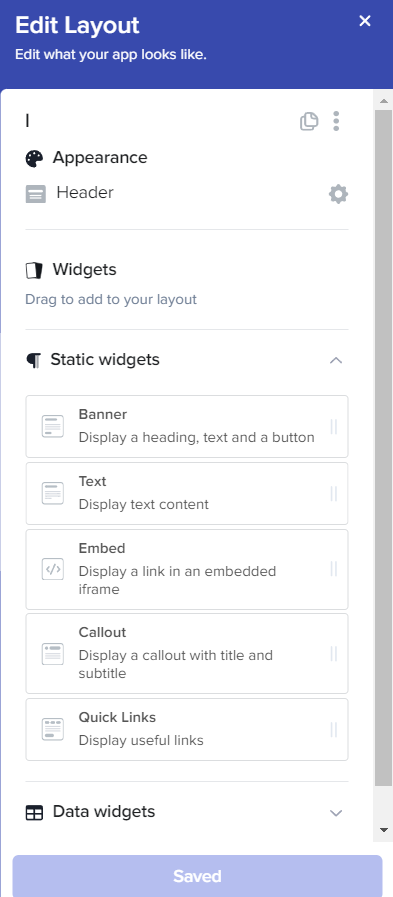
\includegraphics[scale=0.5]{stacker/componenten-stacker1.png}
    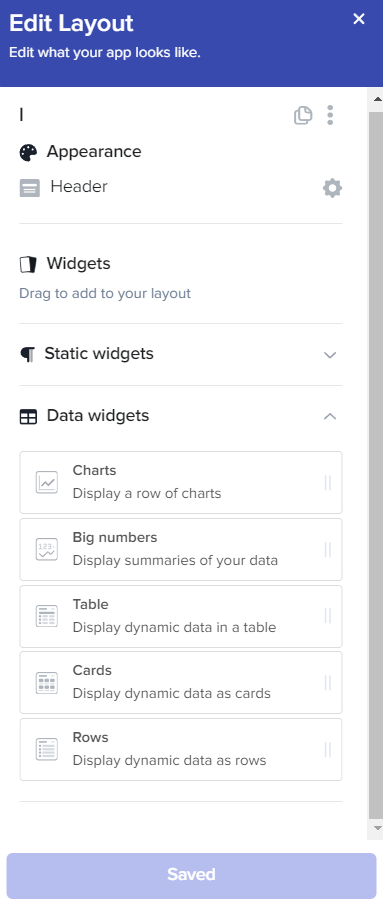
\includegraphics[scale=0.5]{stacker/componenten-stacker2.png}
    \caption[Verschillende componenten in Stacker]{Verschillende componenten in Stacker\\\textcopyright\ Joeri Verhelst}
    \label{fig:componenten-stacker}
\end{figure}
De programmeur vond Stacker gebruiksvriendelijk op bepaalde vlakken. Zo was het connecteren met AirTable zeer eenvoudig en duidelijk.
Ook was het leren van het platform eenvoudig door de duidelijke user interface. Maar in eerste instantie was het wel wat verwarrend om te weten waar je moest beginnen.
Het was namelijk zo dat hij niet wist of dat hij al op het scherm zat voor een app te maken of niet omdat je automatisch al een navigatiebalk hebt.
\\
\\
\paragraph*{Eindresultaat}
Door de zeer beperkte platformflexibiliteit was het namaken van het voorbeeld een grote uitdaging. Hierdoor is het namaken niet gelukt maar hij heeft wel een formulier en homescherm
kunnen ontwikkelen. Tijdens het ontwikkelen was het platform redelijk snel maar de programmeur ervaarden een crash van de laptop bij het snel klikken van verschillende knoppen op het platform.
Deze crash duurde ook ongeveer 30 seconden vooraleer alles terug normaal was. Het totaal ontwikkelen van de app heeft 26 minuten en 47 seconden geduurd. Waarbij het connecteren met AirTable 4 minuten 23 seconden duurde, het ontwikkelen van het formulier 16 minuten en 46,
en het maken van het homescherm 5 minuten en 38 seconden. Hieronder vind u dan ook het eindresultaat van de feedback app.
\\
\\

\begin{figure}[H]
    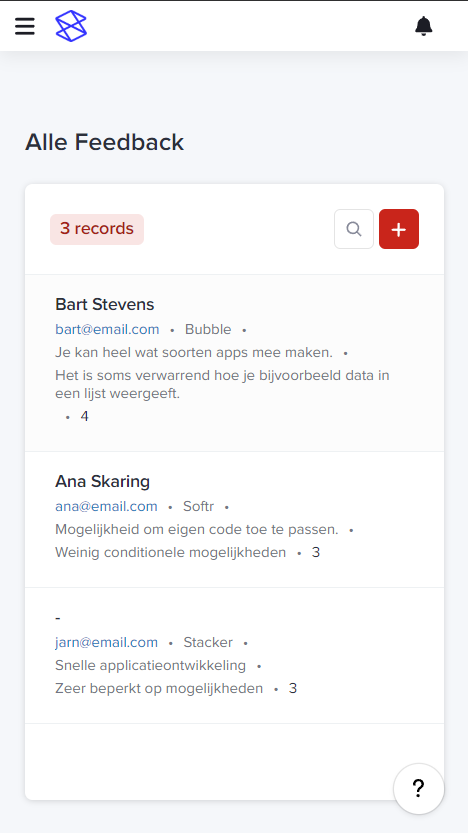
\includegraphics[scale=0.75]{stacker/feedback_lijst.png}
    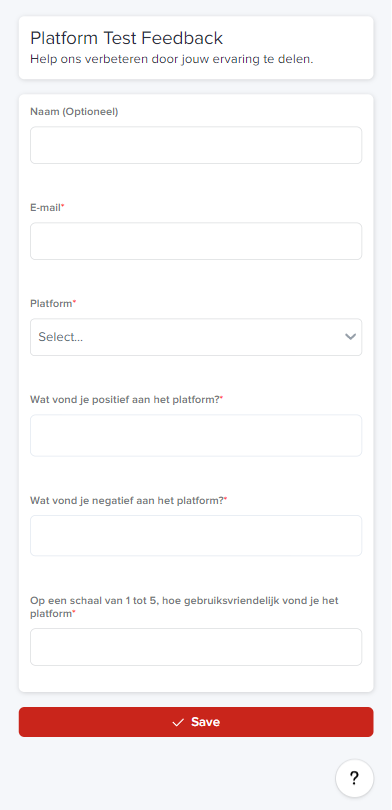
\includegraphics[scale=0.75]{stacker/formulier.png}
    \caption[Feedback app gemaakt in Stacker]{Feedback app gemaakt in Stacker\\\textcopyright\ Joeri Verhelst}
    \label{fig:feedback-app-stacker}
\end{figure}

\paragraph*{Beoordeling}
Door de zeer matige platformflexibiliteit en de beperkte mogelijkheden van apps maken geeft de programmeur Stacker een score van 3 op 5.
De programmeur beveelden dit platform niet aan voor complexe apps te maken, maar eerder voor CRM's en portals.

\subsubsection{Niet-programmeurs}%
\label{subsubsec:niet-programmeurs}
De Proof of Concept voor niet programmeurs, die geen ervaring hebben met programmeren of IT, werd uitgevoerd om 
de gebruiksvriendelijkheid van de platformen te testen. Ter info, deze Proof of Concept is zeer beperkt en is niet voldoende om een definitieve beslissing te nemen over welk platform het beste ervaring geeft voor niet-programmeurs.
\\
\\
\textbf{1. Bubble}
\\
De twee participanten voor Bubble waren Jonas en Marleen. Jonas is begonnen met Bubble als eerste platform waarbij het ongeveer 1u en 25 minuten duurde om de app te maken.
Voor zijn eerste ervaring met zowel een No-Code platform als het platform Bubble vond hij het platform verwarrend. Vervolgens vond hij het gebruiksvriendelijkheid acceptabel doordat het soms
wel zoeken was hoe je iets moest doen. Daarnaast vond hij dat het platform u wel veel mogelijkheden gaf om je app te maken en aan te passen, dit was een reden waarom het juist wat verwarrend was voor hem.
Ten slotte gaf hij het platform een score van 4 op 5 voor hoe goed zijn ervaring was met het platform.
\\
\\
Marleen ondervond verschillende uitdagingen bij het maken van een app in Bubble waarbij zowel de logica als elementen aanpassen moeilijk ging. Hierdoor moest de organisator
regelmatig helpen bij het maken van de app, die ze in ongeveer 1 uur en 30 minuten heeft gemaakt. Ze vond wel dat het platform gebruiksvriendelijk is met hulp maar zonder hulp zou dit niet zo zijn. Ze vond wel een paar dingen positief zoals de vele elemeten die ze kon aanpassen. Daarbij merkte ze ook op 
dat dit platform veel meer biedt dan Stacker. Het enigste waar Marleen niet tevreden overe was het implementeren van logica in de app. Ten slotte gaf ze het platform een score van 2.5 op 5 voor hoe goed haar ervaring was met het platform.
\\
\\
\textbf{2. Softr}
\\
Er waren twee participanten die Softr hebben uitgestest, namelijk Jonas en Ronny. Ronny die begonnen is met Softr als platform heeft een soortgelijke app
gemaakt in ongeveer 1 uur en 15 minuten. Hieruit volgt dat hij meedeelde dat de meeste delen van het platform op eerste instantie niet duidelijk was, maar naarmate de tijd
ging werd het duidelijker. Vervolgens vond hij het platform wel gebruiksvriendelijk waarbij het aanpassen van de indeling zoals kleuren aanpassen zeer eenvoudig was om te toe te passen. Vervolgens heeft Ronny
heel wat moeten vragen aan de organisator.
Ten slotte gaf hij het platform een score van 4 op 5 voor hoe goed zijn ervaring was met het platform.
\\
\\
Jonas heeft voor zijn tweede platform Softr mogen uittesten. In dit platform heeft hij ongeveer 45 minuten gespendeerd om grotendeels de app te kunnen namaken.
Hij vond dat grotendeels alles duidelijk was maar het was soms wel een beetje zoeken. Vervolgens informeerde hij dat het platform gebruiksvriendelijk is, want hij vond het namelijk gemakkelijk om
een vóór opgemaakt lijst of formulier aan te passen naar zijn eigen stijl. Daarbij was er niks negatief aan het platform waardoor hij een score gaf van 5 op 5.
\\
\\
\textbf{3. Stacker}
\\
De participanten voor Stacker waren Ronny en Marleen. Marleen die begonnen is met Stacker als platform heeft ongeveer 1 uur  gespendeerd om de app te proberen namaken, waarbij de organisator regelmatig moest ingrijpen.
In het begin was het moeilijk om te begrijpen voor haar, maar naargelang ze ermee werkte werd het beter. Hieruit volgt dat ze de gebruiksvriendelijkheid niet zo top vond maar vertelde dat het beter zou zijn als ze meer tijd had om het platform te leren kennen.
Ten slotte gaf ze het platform een score van 3 op 5 voor hoe goed haar ervaring was met het platform.
\\
\\
Ronny heeft voor zijn tweede platform Stacker mogen uittesten. In dit platform heeft hij ongeveer 30 minuten gespendeerd om de app te proberen namaken, waarbij de organisator soms moest helpen.
Na een tijdje begon hij het platform beter te begrijpen en vond hij het platform wel gebruiksvriendelijk. Hij vond het namelijk eenvoudig en overzichtelijk om te gebruiken. Ten slotte was zijn ervaring een 
score van 4 op 5 op het platform.

\subsection{Proof of Concept resultaten}%
\label{subsec:proof-of-concept-resultaten}
Door de Proof of Concept kon men verschillende conclusies trekken over de platformen. Hieronder volgt een overzicht van de resultaten van de Proof of Concept.
\\
\\
Bubble scoorde zeer goed op platformflexibiliteit omdat dit kon waargenomen worden door de programmeur maar ook door de twee niet-programmeurs waarbij ze vertelden dat ze veel mogelijkheden hadden om bijvoorbeeld een element aan te passen 
naar hun behoeften. De gebruiksvriendelijkheid was matig waarbij de programmeur het wel goed vond maar had wel meegedeeld dat het soms wel zoeken was hoe je iets moest doen. De twee niet-programmeurs hadden ook moeite met het platform waarbij ze af en toe eens hulp nodig hadden. Vervolgens 
waren de integraties met AirTable en MAKE.com zeer goed en duidelijk. Het maken van een app duurde wel langer dan de andere platformen, maar dit kwam door de vele mogelijkheden dat Bubble biedt.
\\
\\
Softr beschikt over een matige platformflexibiliteit doordat het niet zoveel mogelijkheden heeft als Bubble, maar je kon wel eigen componenten maken. De gebruiksvriendelijkheid was zeer goed volgens de programmeur en de twee niet-programmeurs. Het was eenvoudig en overzichtelijk om te gebruiken.
Daarbij kan men ook hier integreren met MAKE.com of Airtable. Het maken van de app ging sneller dan Bubble.
\\
\\
Stacker is een zeer strikte No-Code platform waarbij je niet veel kan aanpassen. Het had wel een perfecte integratie met Airtable maar kon helaas niet met MAKE.com integreren.
Vervolgens was de gebruiksvriendelijkheid goed maar was eerst verwarrend voor zowel de programmeur als de twee niet-programmeurs. Het maken van de app ging het snelst van de drie platformen.
